\documentclass{article}
\usepackage[a4paper, total={6in, 10in}]{geometry}
\usepackage{graphicx}
\usepackage{hyperref}
\usepackage{listings}
\usepackage{xcolor}
\usepackage{tikz}
\def\checkmark{\tikz\fill[scale=0.4](0,.35) -- (.25,0) -- (1,.7) -- (.25,.15) -- cycle;}
\def \xmark{\tikz\draw[scale=0.4](0,.35) -- (.25,0) -- (1,.7) -- (.25,.15) -- cycle;}

\definecolor{codegreen}{rgb}{0,0.6,0}
\definecolor{codegray}{rgb}{0.5,0.5,0.5}
\definecolor{codepurple}{rgb}{0.58,0,0.82}
\definecolor{backcolour}{rgb}{0.95,0.95,0.92}

\lstdefinestyle{mystyle}{
    backgroundcolor=\color{backcolour},   
    commentstyle=\color{codegreen},
    keywordstyle=\color{magenta},
    numberstyle=\tiny\color{codegray},
    stringstyle=\color{codepurple},
    basicstyle=\ttfamily\footnotesize,
    breakatwhitespace=false,         
    breaklines=true,                 
    captionpos=b,                    
    keepspaces=true,                 
    numbers=left,                    
    numbersep=5pt,                  
    showspaces=false,                
    showstringspaces=false,
    showtabs=false,                  
    tabsize=2
}

\lstset{style=mystyle}
\title{CS221: Operating Systems\\ \Huge Homework 3 Report}
\author{Ali Hamza}
\date{\today}

\begin{document}
\maketitle    
\section{Introduction}
\subsection{Features \& Components}
This homework creates a multithreaded client-server file transfer system. The homework has the following components:
\begin{itemize}
    \item A server that remains open despite the client disconnecting. The server will continue to accept connections and transfer requested files.
    \item The server will be able to clients simultaneously, but this process is not multithreaded.
    \item A client that connects to the server, requests a file, and then remains connected until the user disconnects.
    \item The filetransfer protocol is multithreaded and uses multiple sockets to send the file which achieves data security.
    \item The filetransfer makes sure the empty characters are not being written and the new file created is the same size as the original file.
    \item The codebase contains 4 files:
        \begin{itemize}
            \item \texttt{server.c}
            \item \texttt{server.h}
            \item \texttt{client.c}
            \item \texttt{client.h}
            \item \texttt{helpers.h}
            \item \texttt{makefile}
            \end{itemize}
\end{itemize}
\subsection{Usage}
To compile the code, run the following command in the terminal:
\begin{verbatim}
     make
\end{verbatim}
To run the server, type:
\begin{verbatim}
    ./server <ip> <port>
\end{verbatim}
To run the client, type:
\begin{verbatim}
    ./client <ip> <port>
\end{verbatim}
For example, to run the server and client on the same local machine (\texttt{127.0.0.1}), on port \texttt{8080}, and to request a file named \texttt{test.txt} and save it as \texttt{testNew.txt}, type:
\begin{verbatim}
   ./server 127.0.0.1 8080 (Terminal 1)
   ./client 127.0.0.1 8080 (Terminal 2)
\end{verbatim}
The client will request the user to input: 
\begin{enumerate}
    \item Requested file name
    \item Number of threads to transfer in
    \item Save file as name
\end{enumerate}
The user can disconnect using the \texttt{EXIT} command.
\begin{center}
    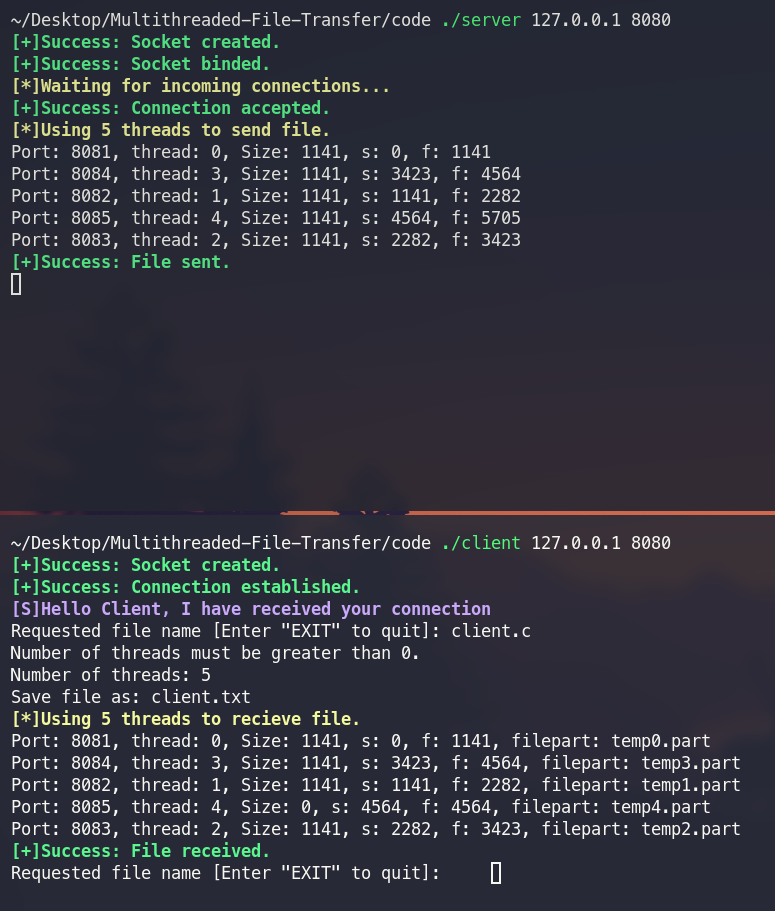
\includegraphics[scale=0.7]{usage.png}
\end{center}
\newpage
\subsection{Functions}
In the \texttt{server.c} file, there are the following functions:
\lstinputlisting[firstline=2, lastline=21, language=c]{server.h}
In the \texttt{client.c} file, there are the following functions, and have the following functionalities.
\lstinputlisting[firstline=2, lastline=22, language=c]{client.h}
In the \texttt{helpers.h} file, there is the struct that is used to pass information to the threads.
\lstinputlisting[firstline = 11, lastline= 20, language=c]{helpers.h}
\newpage
\subsection{Design}
The design of the server is as follows:
\begin{enumerate}
    \item The server will accept connections from n clients.
    \item The client will request a file from the server in \texttt{m} threads
    \item The server will open \texttt{m} ports and send the file to the client in \texttt{m} threads.
    \item The client will recieve the file from the server \texttt{m} ports and write the data to \texttt{m .part} files.
    \item The client will then concatenate the \texttt{.part} files into a new file with the name given by the user.
\end{enumerate}
The below figure shows the server's design.
\begin{figure}[h!]
    \centering
    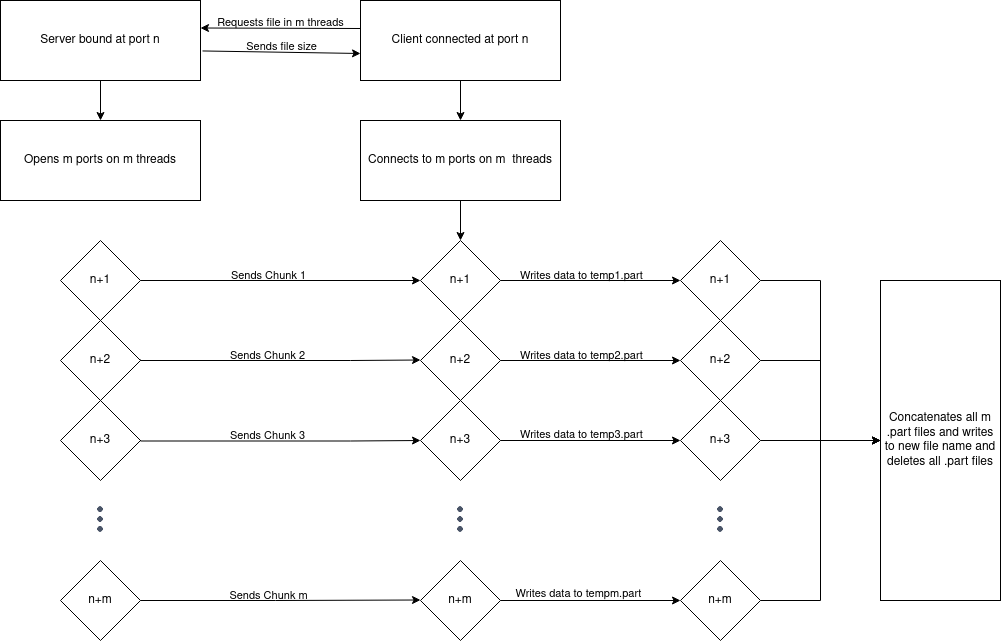
\includegraphics[scale=0.4]{design.png}
    \caption{Server-Client Interaction Design}
\end{figure}
% \newpage
% \section{Testing}
% \begin{enumerate}
%     \item\texttt{Text File: Name:text.txt, Size:11.6 kB}
%     \begin{enumerate}
%         \item \texttt{1 Thread} \checkmark
%         \item \texttt{5 Threads}
%         \item \texttt{10 Threads}
%     \end{enumerate}
%     \item\texttt{Image File: Name:image.jpg, Size:462.1 kB}
%     \begin{enumerate}
%         \item \texttt{1 Thread} \checkmark
%         \item \texttt{5 Threads}
%         \item \texttt{10 Threads}
%     \end{enumerate}
%     \item\texttt{Video File}
%     \begin{enumerate}
%         \item \texttt{1 Thread} \checkmark
%         \item \texttt{5 Threads}
%         \item \texttt{10 Threads}
%     \end{enumerate}
%     \item\texttt{PDF File}
%     \begin{enumerate}
%         \item \texttt{1 Thread} \checkmark
%         \item \texttt{5 Threads}
%         \item \texttt{10 Threads}
%     \end{enumerate}
%     \item\texttt{ZIP File}
%     \begin{enumerate}
%         \item \texttt{1 Thread} \checkmark
%         \item \texttt{5 Threads}
%         \item \texttt{10 Threads}
%     \end{enumerate}
% \end{enumerate}
% \newpage
% \section{Code}
% \subsection{\texttt{server.c}}
% \lstinputlisting[language=c]{server.c}
% \newpage
% \subsection{\texttt{client.c}}
% \lstinputlisting[language=c]{client.c}

\end{document}